\chapter{Introduction to Neural Networks}
\label{sec:neural_networks}

	Artificial Neural Networks take their roots in the structure of the brain and their neurons. In this community, the researchers try to understand and mimic some behaviors of the brain in order to implement what could be named an "artificial-brain". Nowadays, it's believed the brain has a network of neurons triggering signals at at dendrite level and propagating this electrical signal to other neurons through their synapses. Artificial Neural Networks are going to mimic these properties.

	In this chapter we are going to review how artificial neural networks evolved through time, going from the perceptron network, as it was introduced by Rosenblatt in 1958 \cite{rosenblatt1958perceptron} to more modern architecture like the ResNet as submitted by He et al. \cite{he2015deep} in 2015. The first section will describe few neurons : the perceptron, a classic artificial neuron and the recurrent neuron. The second section will describe how to cascade the neurons to build a fully connected neural network and train it. The third section describes CNNs and the last one the uses cases of these networks in classes localization and saliency.
	
	We also introduce some formalism now : As we use them in this thesis, Artificial Neural Network are a way to solve classification tasks. As a reminder, a classification problem that aims at identifying the sub-populations of a set belonging to a class. More specifically: if we are given a set of inputs $X$ and outputs $Y$. where $\boldsymbol{x}^i$ denotes a sample from the set $X$ and $y^i$ its class. Then, the aim of classification is to predict the class of a new sample given the knowledge based on the $\boldsymbol{x}^i$'s.


	\section{Artificial neuron and Perceptron}
	\label{sec:Artificial_neurons}
		The biological neurons are cells that would respond to some electrical inputs emitting or not an electrical response. The artificial neurons mimics theis property numerically. The first artificial neuron we mention here is the \textbf{Perceptron}. It was described by Rosenblatt in 1958 \cite{rosenblatt1958perceptron} and was one of the first artificial neuron introduced in the literature. As all the neurons we'll see here, the neuron first sum its weighted inputs which result in a scalar then apply a transfer function to it. The particularity of the perceptron is its binary inputs and outputs. Once multiplied, its \textit{weighted inputs} are summed-up and if the sum is lower than zero, the neuron outputs zero, Otherwise, the neuron outputs one. A schema of an artificial neuron is given on \Fref{fig:perceptron}.

		Formally: given an input vector $\boldsymbol{x}$ of size $m$ where $x_i$ is the $i$th element of $\boldsymbol{x}$, the Perceptron defines a weight vector $\boldsymbol{w}$ with same shape as the input vector $\boldsymbol{x}$ and a bias term $b$. Then its full function is:

		$$ \text{Perceptron}(x) = \begin{cases}1 & \text{if } \sum_{j=0}^m (w_j \times x_j) + b > 0\\0 & \text{otherwise}\end{cases} $$

		In a vector notation this becomes 

		$$ \text{Perceptron}(x) = \begin{cases}1 & \text{if } \boldsymbol{w}^T \cdot \boldsymbol{x} + b > 0\\0 & \text{otherwise}\end{cases} $$

		Another way of defining the perceptron would be to consider an intermediate value $\boldsymbol{z}=\boldsymbol{w}^T \cdot \boldsymbol{x} + \boldsymbol{b}$ and its transfer function being $\text{Perceptron}(z) = 0 \text{ if } z < 0 \text{ else } 1$. You can visualize this $z$ notation on \fref{fig:neuron_notation}.

		\begin{figure}
			\centering
			\def\layersep{1.5cm}
			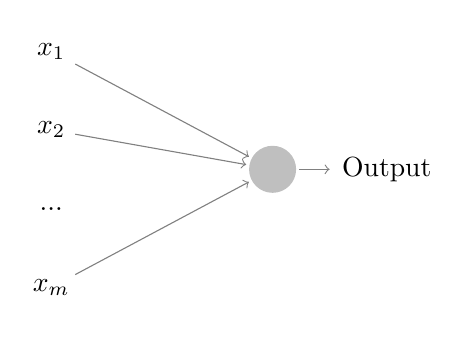
\begin{tikzpicture}[shorten >=1pt,->,draw=black!50, node distance=\layersep]
				\tikzstyle{tata}=[,minimum size=17pt,inner sep=0pt]
			    \tikzstyle{neuron}=[circle,fill=black!25,minimum size=17pt,inner sep=0pt]
			    \tikzstyle{output neuron}=[neuron, fill=red!50];

			    % Input neurons
			    \node[tata] (x1) at (0,-1 cm) {$x_1$};
			    \node[tata] (x2) at (0,-2 cm) {$x_2$};
			    \node[tata] (x3) at (0,-3 cm) {...};
			    \node[tata] (x4) at (0,-4 cm) {$x_m$};
			    
			    % Draw the output layer node
			    \node[neuron,pin={[pin edge={->}]right:Output}] (O) at (\layersep,-2.5) {};

			    % Connect every node in the hidden layer with the output layer
			    \path (x1) edge (O);
			    \path (x2) edge (O);
			    \path (x4) edge (O);

			\end{tikzpicture}
			\caption{Model of an artificial neuron}
			\label{fig:perceptron}
		\end{figure}

		The neurons that appeared later still followed a biologic inspiration as described earlier. Unlike the perceptron, most of these neurons were real-valued and the difference from one to the other resides in its transfer function. We cite here two famous ones :
		\begin{itemize}
			\item The \textbf{sigmoid neuron} which defined by a smooth threshold function:
			$$ \sigma(x) = \frac{1}{1 + e^{-x}} $$
			\item The \textbf{Regression Logistic Unit} (ReLU) which activation function is equal to zero for any negative inputs and equal to its input otherwise. This function got famous with the AlexNet \cite{krizhevsky2012imagenet} where the authors could train a network 4 times quicker than with a usual sigmoid neuron.
			$$ \text{ReLU}(x) = \text{max}(0,x) $$
		\end{itemize}

		Finally, another neuron we'll extensively use in this thesis is the \textbf{Recurrent Neuron}. 


	\section{Neural-network}
		Now that we have neurons, we need a network of them to compose an architecture similar to the brain. The networks we are going to work with are called \textbf{feed-forward} neural-networks. They are the most common ones in the literature. \Fref{fig:feed_forward} is a representation of a two-hidden-layer feed-forward neural-network. As you can see, this model consist of groups of neurons. We denote as layer the group of neurons belonging to the same deepness in the model. Therefore, all the neurons visible on the left in our model, compose the first layer of neurons. It's the input layer. The following layers are called the hidden layers and the last one is the output layer. Some variations exists of this definition, for instance, some outputs of the model might be placed at the same level as some hidden layer.

		Our simple example is also a feed-forward neural-network. It has an input layer fully connected to a hidden layer, which is also fully connected to the output layer. As drawn on the schema with the directions of the arrows, the signal propagates from left to right, from the inputs to the outputs. Because of these two reasons (layers fully connected and single direction signal propagation) our simple example is a feed-forward neural-network.		

		\begin{figure}
			\centering
			\def\layersep{1.5cm}
			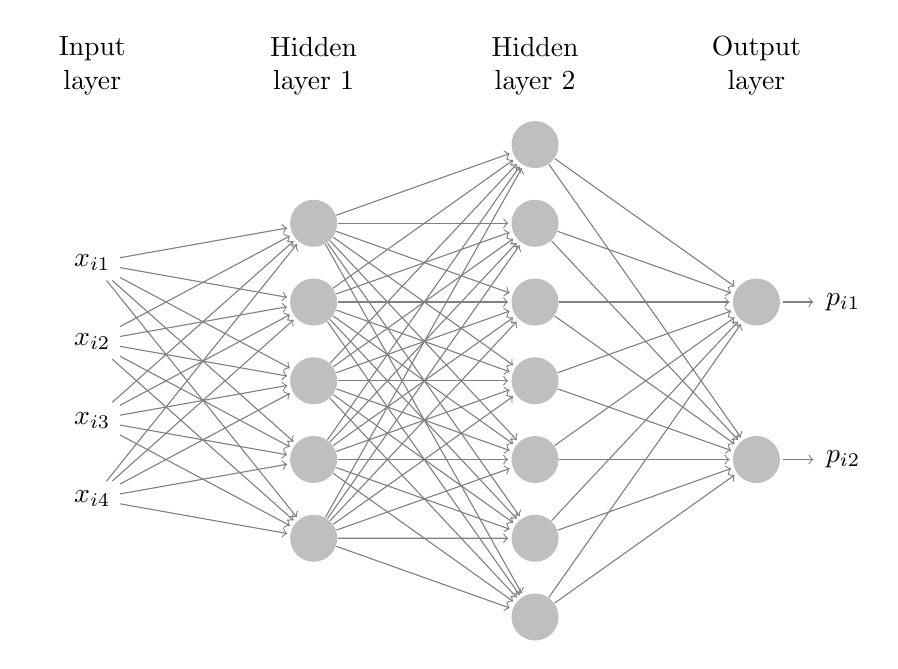
\begin{tikzpicture}[shorten >=1pt,->,draw=black!50, node distance=\layersep]
			    \tikzstyle{every pin edge}=[<-,shorten <=1pt]
			    \tikzstyle{neuron}=[circle,fill=black!25,minimum size=17pt,inner sep=0pt]
			    \tikzstyle{annot} = [text width=4em, text centered]


			    %%%%%%%%%%%%%%%%%%%%%%%%%%%%%%%%%%%%%%%%%%%% 
			    %%% DRAW THE NODES
			    %%%%%%%%%%%%%%%%%%%%%%%%%%%%%%%%%%%%%%%%%%%%
			    \foreach \name / \y in {1,...,4}
			        \node[] (I-\name) at (0,-\y) {$x_{i\y}$};

			    \foreach \name / \y in {1,...,5}
			        \path[yshift=0.5cm] node[neuron] (H1-\name) at (\layersep,-\y cm) {};

				\foreach \name / \y in {1,...,7}
			        \path[yshift=1.5cm] node[neuron] (H2-\name) at (\layersep*2,-\y cm) {};   

		       	
			    \node[neuron,pin={[pin edge={->}]right:$p_{i1}$}, right of=H2-3] (O-1) {};
			    \node[neuron,pin={[pin edge={->}]right:$p_{i2}$}, right of=H2-5] (O-2) {};

			    %%%%%%%%%%%%%%%%%%%%%%%%%%%%%%%%%%%%%%%%%%%% 
			    %%% DRAW THE PATHS
			    %%%%%%%%%%%%%%%%%%%%%%%%%%%%%%%%%%%%%%%%%%%%
			    \foreach \source in {1,...,4}
			        \foreach \dest in {1,...,5}
			            \path (I-\source) edge (H1-\dest);

			    \foreach \source in {1,...,5}
			        \foreach \dest in {1,...,7}
			            \path (H1-\source) edge (H2-\dest);

			    \foreach \source in {1,...,7}
			    	\foreach \dest in {1,...,2}
				        \path (H2-\source) edge (O-\dest);

			    % Annotate the layers
			    \node[annot,above of=H2-1, node distance=1cm] (hl) {Hidden layer 2};
			    \node[annot,left of=hl] (hl1) {Hidden layer 1};
			    \node[annot,left of=hl1] {Input layer};
			    \node[annot,right of=hl] {Output layer};
			\end{tikzpicture}
			\caption{Feed-forward neural-network with two hidden layers}
			\label{fig:feed_forward}
		\end{figure}


		It's good to mention that other types of network exits such as the \textbf{recurrent networks}. In these networks, there is directed cycles on the graph which means that a neuron can depends on its own output. This model is considered to be closer to the brain structure but the challenge on training these models isn't state of the art. We won't work on these models.

		\textbf{Symmetrically connected} networks is an other types of network, they are called the "Boltzmann machines". They are symmetrical in the sense that connections between neurons exists in the two directions and the weight on this connections is the same in both directions. Here again, we won't work on these models.


	\section{Forward-propagation}
	\label{sec:forward_propagation}
		The logic route now is to relate our neural-network to the prediction or classification task. Lets consider we have a neural-network. This neural-network has weight vectors and biases initialized for each of its neurons. When we input a vector on the left of this neural-network each neurons on the next layer will be assigned a local output value (given the inputs on the previous layer). Following this same pattern from layer to layer, the input signal (vector $\boldsymbol{x}$) will propagate until the output layer resulting in our prediction.

		\vskip 1cm
		\textit{\textbf{Notation:}}
		To refer to the weights of the $j$th neuron of the $l$th layer we note $\boldsymbol{w}^l_j$. The superscript refer to the layer and the lower-script refer to the neuron number on this layer. Also, we note $b^l_j$ the bias of the $j$th neuron of the $l$th layer. As a sum-up of the inputs, $z^l_j$ is the weighted sum plus bias (${\boldsymbol{w}^l_j}^T x + b^l_j$) of the $j$th neuron of the $l$th layer. Finally, the output of neuron $j$ on layer $l$ is denoted $a^l_j$. \Fref{fig:neuron_notation} sums-up these notations.
		Instead of referring to each and every vectors, we often refer to the matrices composed by the vectors. For instance $W^i$ is the weight matrix composed by each neuron's vectors of the $l$th layer.
		\begin{figure}
			\centering
			\def\layersep{8em}	
			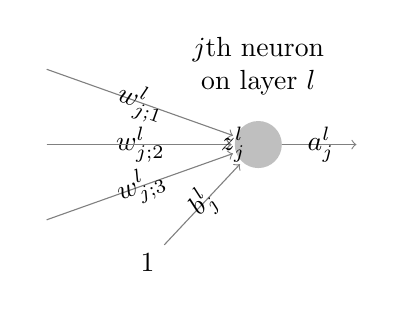
\begin{tikzpicture}[shorten >=1pt,->,draw=black!50, node distance=\layersep]
			    \tikzstyle{every pin edge}=[<-,shorten <=1pt]
			    \tikzstyle{pixel} = []
			    \tikzstyle{neuron}=[circle,fill=black!25,minimum size=17pt,inner sep=0pt]
			    \tikzstyle{annot} = [text width=2em, text centered]
			    \tikzstyle{annot2} = [text width=6em, text centered]
			    
			    %%% DRAW THE NODES
			    \foreach \name / \y in {1,...,3}
			        \node[pixel] (I-\name) at (0,-\y) {};
			    \node (I-4) at (\layersep*.5,-3.5) {$1$};
				\node[neuron] (H-1) at (\layersep*1,-2) {};
				\node[pixel] (O-1) at (\layersep*1.5,-2) {};


			    %%% DRAW THE PATHS
	            \path[every node/.style={sloped}] (I-1) edge node[annot]  {$ w^l_{j;1} $} (H-1);
	            \path[every node/.style={sloped}] (I-2) edge node[annot]  {$ w^l_{j;2} $} (H-1);
	            \path[every node/.style={sloped, anchor=west}] (I-2) edge node[annot2] {$ z^l_j     $} (H-1);
	            \path[every node/.style={sloped}] (I-3) edge node[annot]  {$ w^l_{j;3} $} (H-1);
	            \path[every node/.style={sloped}] (I-4) edge node[annot]  {$ b^l_j   $} (H-1);

	            \path[every node/.style={sloped}] (H-1) edge node[annot]  { $a^l_j$ } (O-1);

			    %%% ANOTATE
			    \node[annot2,above of=H-1, node distance=1cm] () {$j$th neuron on layer $l$};

			\end{tikzpicture}
			\caption{Our notation in a neuron}
			\label{fig:neuron_notation}
		\end{figure}

		\vskip 1cm
		Lets demonstrate this forward-propagation on our simple example. We will propagate $\boldsymbol{x}^1$, the first input sample of the dataset, and get the prediction made by the network. To do so, we need to initialize the weights and biases of the 6 neurons we have. We use weight initialization written on table\ref{tab:NN_weights}.

		\begin{table}[ht]
			\centering
			\begin{tabular}{c|c|c||c|c|c}
				$\boldsymbol{w}^1_1$ & $\boldsymbol{w}^1_2$ & $\boldsymbol{w}^1_3$ & $\boldsymbol{w}^2_1$ & $\boldsymbol{w}^2_2$ & $\boldsymbol{w}^2_3$ \\
				\hline
					$ \left( \begin{matrix} -10  \\ -10  \\  20 \end{matrix}\right) $ &
					$ \left( \begin{matrix} -10  \\  10  \\  10 \end{matrix}\right) $ &
					$ \left( \begin{matrix}  10  \\ -10  \\  10 \end{matrix}\right) $ &
					$ \left( \begin{matrix}  5   \\ -5   \\ -5  \end{matrix}\right) $ &
					$ \left( \begin{matrix} -5   \\  5   \\ -5  \end{matrix}\right) $ &
					$ \left( \begin{matrix} -5   \\ -5   \\  5  \end{matrix}\right) $ \\
				\hline
				\hline
				$b^1_1$ & $b^1_2$ & $b^1_3$ & $b^2_1$ & $b^2_2$ & $b^2_3$ \\
				$-13$   & $-13$   & $-13$   & $0$     & $0$     & $0$     \\
			\end{tabular}
			\caption{ \fref{fig:simple_NN_init} shows the weights on a schema}
			\label{tab:NN_weights}
		\end{table}

		Given these weights, retrieving the prediction of the class of $\boldsymbol{x}^1$ consists on: 
		\begin{itemize}
			\item Propagating $\boldsymbol{x}^1$ through the first neuron layer:
			$$ \sigma(\boldsymbol{z}^1) = \sigma({\boldsymbol{W}^1}^T \boldsymbol{x}^1 + \boldsymbol{b}^1) $$
			$ \sigma \left(
			\left( \begin{matrix} -10 & -10 & 20 \\ -10 & 10 & 10 \\ 10 & -10 & 10 \end{matrix}\right) \cdot
			\left( \begin{matrix} 0  \\ 0  \\ 1  \end{matrix}\right) +
			\left( \begin{matrix} -13 \\ -13 \\ -13 \end{matrix}\right) \right) = 
			\sigma \left( 
			\left( \begin{matrix} 7 \\ -3 \\ -3 \end{matrix}\right) \right) = 
			\left( \begin{matrix} .999 \\ .047 \\ .047 \end{matrix}\right) $
			\item Propagating $\sigma(\boldsymbol{z}^1)$ through the second neuron layer (the prediction layer):
			$$ p(\boldsymbol{z}^1) = \sigma({\boldsymbol{W}^2}^T \sigma(\boldsymbol{z}^1) + \boldsymbol{b}^2) $$
			$ \sigma \left(
			\left( \begin{matrix} 5 & -5 & -5 \\ -5 & 5 & -5 \\ -5 & -5 & 5 \end{matrix}\right) \cdot
			\left( \begin{matrix} .999  \\ .047  \\ .047  \end{matrix}\right) +
			\left( \begin{matrix} 0 \\ 0 \\ 0 \end{matrix}\right) \right) = 
			\sigma \left( 
			\left( \begin{matrix} 9.042 \\ -9.991 \\ -9.991 \end{matrix}\right) \right) = 
			\left( \begin{matrix} .989 \\ .007 \\ .007 \end{matrix}\right) $
		\end{itemize}

		We have here the prediction for $\boldsymbol{x}^1$. To have a percentage out of this prediction we normalize prediction and get that sample $\boldsymbol{x}^1$ could be of class 1 with $98,6\%$ accuracy, could be of class 2 with $.7\%$ or of class 3 with $.7\%$ accuracy. Our simple example, initialized with these weights made an accurate prediction for this sample.
	

	\section{Cost function}
	\label{sec:cost_function}
		Once we have build our model, we consider a cost function, also called "loss function". This cost function define how good is the model doing, considering an evaluation criterion. In the case of classification, we want to evaluate how good the prediction is doing towards the true output.
		The most famous cost functions in neural-network classification are the squared error and the cross entropy (also called the "negative log-likelihood"). For a given sample $i$ with prediction $\boldsymbol{p}^i$ and the true output $\boldsymbol{y}^i$, they are defined as follow:
		\begin{itemize}
			\item Squared error: $$ l(\boldsymbol{p}^i,\boldsymbol{y}^i) = \norm{\boldsymbol{y}^i - \boldsymbol{p}^i}_2^2 $$
			\item Cross entropy: $$ l(\widetilde{\boldsymbol{p}^i},\boldsymbol{y}^i) = -\ln(\widetilde{\boldsymbol{p}^i})^T\cdot{\boldsymbol{y}^i}  $$
		\end{itemize}
		Where $ \tilde{p} $ is the normalized value of the prediction over all the predictions. To evaluate the error of the entire dataset, we use the mean of all the errors. $l(\boldsymbol{P},\boldsymbol{Y}) = \sum_i l(\boldsymbol{p}^i,\boldsymbol{y}^i)$

		\vskip 1cm
		We are going to compute these two errors for the sample one but later on the report, we will only consider the cross entropy.
		\begin{itemize}
			\item Squared error: $$ l(\boldsymbol{p}^1,\boldsymbol{y}^1) =  
									\norm{
									\left( \begin{matrix} .989 \\ .007 \\ .007 \end{matrix}\right) - 
									\left( \begin{matrix} 1    \\ 0    \\ 0    \end{matrix}\right) }_2^2 = 
									.011^2 + .007^2 + .007^2 = .021 $$
			\item Cross entropy: $$ l(\widetilde{\boldsymbol{p}^1},\boldsymbol{y}^1) = 
									- \ln
								 	\widetilde{\left( \begin{matrix} .989 \\ .007 \\ .007 \end{matrix}\right)}^T \cdot 
									\left( \begin{matrix} 1    \\ 0    \\ 0    \end{matrix}\right) = 
									- \ln
								 	\left( \begin{matrix} .986 \\ .007 \\ .007 \end{matrix}\right)^T \cdot 
									\left( \begin{matrix} 1    \\ 0    \\ 0    \end{matrix}\right) = 
									-\ln(.986) = .011
									$$
		\end{itemize}
		
		For the rest of the thesis, we'll be using the cross entropy error function. There is no special motivation under this choice. One mustn't believe that this choice is motivated by $.011$ being lower than $.021$. This result comes from the fact that there are two distinct costs. One compares a distance to the true output (the squared error) whereas cross-entropy gives a negative-log-likelihood.


	\section{Back-propagation}
	\label{sec:back_propagation}
		Until now we've seen how to build a model. We initialized our model with some specific values and propagated an input through this model. The forward-propagation of the signal gave us a prediction that could be compared to the true prediction of the sample thank to a cost function. Given an entire test set, we could use the same cost function to evaluate our model. In this subsection and the following, we investigate on how to modify the model such that it performs better.

		\subsection{Intuition}
			We want the model to perform better. We can't change the input samples nor their true predictions. The only parameters we can change are in the model. We could add neurons and see how new neurons improve the current model but we don't. What we are going to do is to modify the neurons such that they have a positive impact on the error. For each neurons present on the model, we are going to see how a twist on their weights and biases impacts the error made by the model. To find the good twists we use Back-propagation and to take a step in the direction of this twist we use gradient descent (section \ref{sec:gradient_desent}).

			The name of back-propagation comes as the opposite of forward-propagation. We start from the cost ($C=l(\boldsymbol{P},\boldsymbol{Y})$) of the network and see how twisting the weights of the neurons, layer after layers, affects the cost. To be more formal, we search for the direction of the derivative of the cost as a function of the weights and biases of neuron $j$ on layer $i$. To reach this step, we will first consider $\delta^l_i$, the derivative of the cost with respect to the input of neuron $j$ of layer $l$.
			$$ \delta^l_j = \frac{\partial C}{\partial z^l_j } $$
			You might want to watch \fref{fig:neuron_notation} to remind the notation. Also, for notation convenience we'll be using many vector/matrix notations. As a result, we'll use the Hadamard ("$\circ$") and the Kronecker ("$\otimes$") products. The definitions of these two products are reminded in appendix \ref{sec:hadamar_product}.

		\subsection{Step-by-step}
			The \textbf{first} step of back-propagation is to back-propagate the cost $C$ to the last layer $L$.

			\begin{tabular}{c|c}
				\parbox{14em}{
					\begin{equation}
						\begin{split}
							\delta^L_i
							&= \frac{\partial C}{\partial z^L_i } \\
							&= \frac{\partial a^L_i }{\partial z^L_i } \cdot \frac{\partial C}{\partial a^L_i }
						\end{split}
					\end{equation}
				}
				& \parbox{14em}{
					\begin{equation}
						\begin{split}
							\boldsymbol{\delta}^L
							&= \frac{\partial C}{\partial \boldsymbol{z}^L } \\
							&= \frac{\partial \boldsymbol{a}^L }{\partial \boldsymbol{z}^L } \circ \frac{\partial C}{\partial \boldsymbol{a}^L }
						\end{split}
					\end{equation}
				}
			\end{tabular}

			On this last equation, we see that deriving the cost with respect to the neurons' inputs of the last layer $L$ consist on deriving the cost $C$ with respect to the prediction $p$ and on deriving the output of a neuron with respect to it's inputs. 

			The \textbf{second} step is to back-propagate the cost to the other layers $l$. We will here take advantage of the chain rule. 
			\begin{equation}
				\begin{split}
					\boldsymbol{\delta}^l
					&=  \frac{\partial C}{\partial \boldsymbol{z}^l } \\
					&=	\left(\frac{\partial \boldsymbol{a}^l }{\partial \boldsymbol{z}^l }  					\circ\frac{\partial \boldsymbol{z}^{l+1} }{\partial \boldsymbol{a}^l } \right) 	\cdot
					\left(\frac{\partial \boldsymbol{a}^{l+1} }{\partial \boldsymbol{z}^{l+1} }  		\circ\frac{\partial \boldsymbol{z}^{l+2}}{\partial \boldsymbol{a}^{l+1} }\right)  (...)
					\left(\frac{\partial \boldsymbol{a}^L }{\partial \boldsymbol{z}^L } 		 		\circ\frac{\partial C}{\partial \boldsymbol{a}^L }\right) \\
					&=  \left(\frac{\partial \boldsymbol{a}^l }{\partial \boldsymbol{z}^l }  					\circ\frac{\partial \boldsymbol{z}^{l+1} }{\partial \boldsymbol{a}^l }  \right) \cdot
						\left( \frac{\partial \boldsymbol{a}^{l+1} }{\partial \boldsymbol{z}^{l+1} }  	\circ\frac{\partial \boldsymbol{z}^{l+2}}{\partial \boldsymbol{a}^{l+1} }\right) (...)
						\left( \frac{\partial \boldsymbol{a}^L }{\partial \boldsymbol{z}^L }			\circ\frac{\partial C}{\partial \boldsymbol{a}^L }\right) \\
					&= 	\left(\frac{\partial \boldsymbol{a}^l }{\partial \boldsymbol{z}^l }   				\circ\frac{\partial \boldsymbol{z}^{l+1} }{\partial \boldsymbol{a}^l } \right) 		\cdot
						\left( \frac{\partial \boldsymbol{a}^{l+1} }{\partial \boldsymbol{z}^{l+1} }  	\circ\frac{\partial \boldsymbol{z}^{l+2}}{\partial \boldsymbol{a}^{l+1} }\right) (...) 
						\boldsymbol{\delta}^{L}\\
					&= 	\left(\frac{\partial \boldsymbol{a}^l }{\partial \boldsymbol{z}^l }  					\circ\frac{\partial \boldsymbol{z}^{l+1} }{\partial \boldsymbol{a}^l } \right) 	\cdot
						\boldsymbol{\delta}^{l+1}
				\end{split}
			\end{equation}
			At the very end of this equation we see how deriving the cost $C$ with respect to the inputs of layer $l$ depends on the derivative of the next layer, and therefore how back-propagation occurs.

			The \textbf{third} part of the algorithm consist on deriving the cost $C$ with respect to the weights $\boldsymbol{w}^l_j$ and biases $b^l_j$.

			\begin{tabular}{c|c}
				\parbox{14em}{
					\begin{equation}
						\begin{split}
							\frac{\partial C}{\partial \boldsymbol{w}^l_j}
							&= \frac{\partial z^l_j}{\partial \boldsymbol{w}^l_j} \frac{\partial C}{\partial z^l_j} \\
							&= \frac{\partial z^l_j}{\partial \boldsymbol{w}^l_j} \delta^l_j \\
						\end{split}
					\end{equation}
				}
				& \parbox{14em}{
					With $\boldsymbol{z}^l = \boldsymbol{W}^{lT} \boldsymbol{a}^{l-1} + \boldsymbol{b}^l $
					\begin{equation}
						\begin{split}
							\frac{\partial C}{\partial \boldsymbol{W}^l}
							&= \frac{\partial \boldsymbol{z}^l}{\partial \boldsymbol{W}^l} \otimes \frac{\partial C}{\partial \boldsymbol{z}^l} \\
							&= \frac{\partial \boldsymbol{z}^l}{\partial \boldsymbol{W}^l} \otimes {\boldsymbol{\delta}^l} \\
							&= \boldsymbol{a}^{(l-1)T} \otimes \boldsymbol{\delta}^l \\
						\end{split}
					\end{equation}
				}
			\end{tabular}
			\vskip 1em
			\begin{tabular}{c|c}
				\parbox{14em}{
					\begin{equation}
						\begin{split}
							\frac{\partial C}{\partial b^l_j}
							&= \frac{\partial z^l_j}{\partial b^l_j} \frac{\partial C}{\partial z^l_j} \\
							&= \frac{\partial z^l_j}{\partial b^l_j} \delta^l_j \\
						\end{split}
					\end{equation}
				} & \parbox{14em}{
					With $\boldsymbol{z}^l = \boldsymbol{W}^{lT} \boldsymbol{a}^{l-1} + \boldsymbol{b}^l $
					\begin{equation}
						\begin{split}
							\frac{\partial C}{\partial \boldsymbol{b}^l}
							&= \frac{\partial \boldsymbol{z}^l}{\partial \boldsymbol{b}^l} \otimes \frac{\partial C}{\partial \boldsymbol{z}^l} \\
							&= \boldsymbol{\delta}^l \\
						\end{split}
					\end{equation}
				}
			\end{tabular}



		\subsection{Equations applied to our simple example}
			Before applying the back-propagation, we are going to compute some important derivatives. We will differentiate our cross entropy cost $C$ with respect to its inputs and differentiate the sigmoid neurons with respect to their inputs too.
			\begin{itemize}
				\item The \textbf{derivative of the cost} $C$ with respect to the predictions $p_j$:
					\begin{equation}
						\begin{split}
							\frac{\partial C}{\partial a^L_j}
							&= \frac{\partial C}{\partial p_j} \\
							&= \frac{\partial \left( -\ln(\boldsymbol{p})^T \cdot \boldsymbol{y} \right) }{\partial p_j} \\
							&= -\sum_k \left( \frac{y_k \partial \ln(p_k)}{\partial p_k}\frac{\partial p_k}{\partial p_j} \right)\\
							&= -\sum_k \left( \frac{y_k}{p_k}\frac{\partial p_k}{\partial p_j} \right)\\
						\end{split}
					\label{eq:cost_over_pred}
					\end{equation}
				\item The \textbf{derivative of a neuron}'s output $a^l_j$ with respect to its inputs $z^l_j$ (or $\boldsymbol{a}^l$ wrt. $\boldsymbol{z}^l$).
					\vskip 1em
					\begin{tabular}{c|c}
						\parbox{14em}{
							\begin{equation}
								\begin{split}
									\frac{\partial a^l_j}{\partial z^l_j}
									&= \frac{\partial \sigma(z^l_j)}{\partial z^l_j} \\
									&= a^l_j (1-a^l_j)
								\end{split}
							\end{equation}
						}& \parbox{14em}{
							\begin{equation}
								\begin{split}
									\frac{\partial \boldsymbol{a}^l}{\partial \boldsymbol{z}^l}
									&= \frac{\partial \sigma(\boldsymbol{z}^l)}{\partial \boldsymbol{z}^l} \\
									&= \boldsymbol{a}^l \circ (1-\boldsymbol{a}^l)
								\end{split}
							\end{equation}
						}
					\end{tabular}
				\item \textbf{Derivative of the softmax neurons}: In the cost description (section \ref{sec:cost_function}), we mention a normalized input $\widetilde{\boldsymbol{p}}$ but didn't emphasize on it. This normalized input impacts the last layer of the network such that the derivatives of this layer are different than simple sigmoid neurons. That kind of layer is called a softmax layer and is often used when neural-networks when dealing with multi-class tasks. You'll find more information on this function on the "Pattern recognition and machine learning" book \cite{bishop2006pattern} starting on page 113. Right bellow we derive the outputs of these softmax neurons with their aggregated inputs. There is two cases to derive: the first one is when we differentiate the neuron $a^L_j$ with respect to $z^L_j=1$. The second is when we derive the other neurons $a^L_j$ with respect to $z^L_m=0$.
				\begin{itemize}
					\item If $p_j$ is derived from its input $z^L_j$
						\begin{equation}
							\label{eq:softmax_deriv_1}
							\begin{split}
								\frac{\partial a^L_j}{\partial z^L_j}
								&= \frac{\partial p_j}{\partial z^L_j} \\
								&= \frac{\partial (e^{z^L_j}/\sum_k e^{z^L_k})}{ \partial z^L_j} \\
								&= p_j (1-p_j)
							\end{split}
						\end{equation}
					\item IIf $p_j$ is derived from another input $z^L_m$
						\begin{equation}
							\label{eq:softmax_deriv_2}
							\begin{split}
								\frac{\partial a^L_j}{\partial z^L_m}
								&= \frac{\partial p_j}{\partial z^L_m}\\
								&= \frac{\partial (e^{z^L_m}/\sum_k e^{z^L_k})}{ \partial z^L_j} \\
								&= -p_j p_m
							\end{split}
						\end{equation}
				\end{itemize}
			\end{itemize}

			\vskip 1cm
			\textbf{Back-propagate:}\\
			We've seen the result of some derivatives of some functions present in our simple example. These derivatives will help us in applying the back-propagation algorithm. As mentions on the previous section, there is three main steps to take. \textbf{First} differentiate the cost $C$ with respect to the inputs of the last layer. In our case we differentiate the cross entropy function with respect to the inputs of normalized-output-neurons. In other words we derive the cost function with respect to the inputs of the softmax neurons. The \textbf{second} step consist on back-propagating the error layer by layer such that we get the derivative of the cost with respect to the inputs of layer $l$. \textbf{Third}, and last step, is to compute the derivatives at the weights and biases level instead of just the 'input' of the neurons as we've been doing so far.
			\begin{enumerate}
				\item To compute the \textbf{derivative of the cost} with respect to the inputs of the \textbf{softmax layer} we use the results of equations \ref{eq:cost_over_pred}, \ref{eq:softmax_deriv_1} and \ref{eq:softmax_deriv_2}.
					\begin{equation}
						\begin{split}
							\delta^L_j
							&= \frac{\partial C}{\partial z^L_j } \\
							&= \frac{\partial C}{\partial p_j} \frac{\partial p_j}{\partial z^L_j } \\
							&= -\left(\sum_k \frac{y_k}{p_k} \cdot \frac{\partial p_k}{\partial p_j } \frac{\partial p_j}{\partial z^L_j } \right) \\
							&= -\left(\sum_k \frac{y_k}{p_k} \cdot \frac{\partial p_k}{\partial z^L_j } \right) \\
							&= -\left(\sum_{k=j} \frac{y_k}{p_k} \cdot p_k(1 - p_k) \right) - \left(\sum_{k!=j} \frac{y_k}{p_k} \cdot -(p_j p_k) \right) \\
							&= -\left(y_j  (1 - p_j) \right) + \left(\sum_{k!=j} y_k(p_j) \right) \\
							&=  \left(y_j p_j  - y_j\right)  + \left(\sum_{k!=j} y_k p_j  \right) \\
							&=  \left(\sum_{k} y_k p_j  \right) - y_j \\
							&=  p_j - y_j \\
						\end{split}
					\end{equation}
					Which in a vector notation is $\boldsymbol{\delta}^L = \boldsymbol{p} - \boldsymbol{y}$
				\item Then we \textbf{back-propagate} to other layers. We only have two layers, we've just done the last layer $l=2$. We now do layer $l=1$
					\begin{equation}
						\begin{split}
							\boldsymbol{\delta}^{1}
							&= \frac{\partial \boldsymbol{a}^1 }		{\partial \boldsymbol{z}^1 } 		\circ
							\left( \frac{\partial \boldsymbol{z}^2 }	{\partial \boldsymbol{a}^1 } \cdot \boldsymbol{\delta}^2 \right) \\
							&= \frac{\partial \sigma(\boldsymbol{z}^1)}	{\partial \boldsymbol{z}^1}\circ
							\left( \frac{\partial ({\boldsymbol{W}^2}^T \boldsymbol{a}^1 + \boldsymbol{b}^1 )}{\partial \boldsymbol{a}^1} \cdot \boldsymbol{\delta}^2 \right)\\
							&= \sigma(\boldsymbol{z}^1)\circ(1-\sigma(\boldsymbol{z}^1)) \circ ({\boldsymbol{W}^2}^T \cdot \boldsymbol{\delta}^2) \\
							&= \boldsymbol{a}^1 \circ(1-\boldsymbol{a}^1) \circ ({\boldsymbol{W}^2}^T \cdot \boldsymbol{\delta}^2) \\
						\end{split}
					\end{equation}
				\item Finally, we compute the \textbf{derivative of the costs} with respect to the \textbf{weights and biases}.\\
				\begin{tabular}{c|c}
					\parbox{14em}{
						\begin{equation}
							\begin{split}
								\frac{\partial C}{\partial \boldsymbol{W}^2}
								&= \frac{\partial \boldsymbol{z}^2}{\partial \boldsymbol{W}^2} \otimes {\boldsymbol{\delta}^2} \\
								&= {\boldsymbol{a}^1}^T \otimes {(\boldsymbol{p} - \boldsymbol{y})} \\
							\end{split}
							\label{eq:BP_w2}
						\end{equation}
					} & \parbox{14em}{
						\begin{equation}
							\begin{split}
								\frac{\partial C}{\partial \boldsymbol{W}^1}
								&= \frac{\partial \boldsymbol{z}^1}{\partial \boldsymbol{W}^1} \otimes {\boldsymbol{\delta}^1} \\
								&= \boldsymbol{x}^T \otimes {\boldsymbol{\delta}^1} \\
							\end{split}
							\label{eq:BP_w1}
						\end{equation}
					} \\
					\parbox{14em}{
						\begin{equation}
							\begin{split}
								\frac{\partial C}{\partial \boldsymbol{b}^2}
								&= \frac{\partial \boldsymbol{z}^2}{\partial \boldsymbol{b}^2} \otimes {\boldsymbol{\delta}^2} \\
								&= (\boldsymbol{p} - \boldsymbol{y}) \\
							\end{split}
							\label{eq:BP_b2}
						\end{equation}
					} & \parbox{14em}{
						\begin{equation}
							\begin{split}
								\frac{\partial C}{\partial \boldsymbol{b}^1}
								&= \frac{\partial \boldsymbol{z}^1}{\partial \boldsymbol{b}^1} \otimes {\boldsymbol{\delta}^1} \\
								&= \boldsymbol{\delta}^1 \\
							\end{split}
							\label{eq:BP_b1}
						\end{equation}
					}
				\end{tabular}
			\end{enumerate}




	\section{Gradient descent}
	\label{sec:gradient_desent}
		With back-propagation, we've computed the derivatives of the cost with respect to the weights and biases of the model. In other words, we've seen how to twist the neurons' parameters such that, given an input sample, they lower the cost.

		We now want to find the neurons' parameters that will lower the model's cost $C$. We'll search for this value with Gradient Descent. Gradient descent is an iterative algorithm aiming at finding the local minimums of a function. At each steps its improves its chances to be closer to a local minimum.

		\vskip 1em
		Consider a function $f:\mathbb{R}^n\rightarrow\mathbb{R}$ and its gradient $\nabla f$. Gradient descent works by taking advantage of the gradient of the function $f$ at a point $x$ such that, following the negative value of the gradient, the algorithm can find a local minimum for the function. 
		$$ x_{t+1} = x_t - \epsilon \nabla f(x)$$


		On deep learning, we don't use gradient descent but \textbf{Stochastic Gradient Descent (SGD)}. This descent algorithm picks a sample at random on the dataset and evaluate the gradient from it. Still, ”The derivative based on a randomly chosen single example is a random approximation to the true derivative based on all the training data” \cite{elkan2013maximum}.


		\subsection{Example on our simple example}
			We want to perform a step towards a lower cost on our simple example using SGD. We'll pick 'at random' the 1st sample on the training set:
			$$ \boldsymbol{x}^1 = \left( \begin{matrix} 0  \\ 0  \\ 1  \end{matrix}\right) $$
			That is of class $y^1 = 1$. The model we consider is initialized as before. It has the weight and biases of \fref{tab:NN_weights}.

			To perform a step toward a lower cost in the model, we use the prediction made by the current model on this sample $\boldsymbol{x}^1$ (already computed on section \ref{sec:forward_propagation}), and compute the back-propagation equation \ref{eq:BP_w2}, \ref{eq:BP_w1}, \ref{eq:BP_b2}, \ref{eq:BP_b1} with the prediction $\boldsymbol{p}^1$ and output $\boldsymbol{y}^1$.

			Using an epsilon $\epsilon = .5$, we get the following updates : 


			\begin{tabular}{cc}
				$ \boldsymbol{W}^1_{t+1} = \boldsymbol{W}^1_t - \epsilon \frac{\partial C}{\partial \boldsymbol{W}^1} = 
					\left( \begin{matrix}
					-10.0 	& -10.0 	& 10.0 \\
					-10.0 	& 10.0 	& -10.0 \\
					20.0 	& 10.0 	& 10.0 \\
					\end{matrix} \right) - \epsilon 
					\left( \begin{matrix}
					-0.0 	& 0.0 	& 0.0 \\
					-0.0 	& 0.0 	& 0.0 \\
					-0.0 	& 0.003 	& 0.003 \\
					\end{matrix} \right) $ \\
				$ \boldsymbol{W}^1_{t+1} = 
					\left( \begin{matrix}
					-10.0 	& -10.0 	& 10.0 \\
					-10.0 	& 10.0 		& -10.0 \\
					20.0 	& 9.998 	& 9.998 \\
					\end{matrix} \right)$ \\

				\hline
				$ \boldsymbol{W}^2_{t+1} = \boldsymbol{W}^2_t - \epsilon \frac{\partial C}{\partial \boldsymbol{W}^2} = 
					\left( \begin{matrix}
					5.0 	& -5.0 	& -5.0 \\
					-5.0 	& 5.0 	& -5.0 \\
					-5.0 	& -5.0 	& 5.0 \\
					\end{matrix} \right) - \epsilon 
					\left( \begin{matrix}
					-0.013 	& 0.007 	& 0.007 \\
					-0.001 	& 0.0 	& 0.0 \\
					-0.001 	& 0.0 	& 0.0 \\
					\end{matrix} \right) $ \\
				$ \boldsymbol{W}^2_{t+1} = 
					\left( \begin{matrix}
					5.007 	& -5.003 	& -5.003 \\
					-5.0 	& 5.0 	& -5.0 \\
					-5.0 	& -5.0 	& 5.0 \\
					\end{matrix} \right)$ \\


				\hline
				$ \boldsymbol{b}^1_{t+1} = \boldsymbol{b}^1_t - \epsilon \frac{\partial C}{\partial \boldsymbol{b}^1} = 
					\left( \begin{matrix}
					-13.0 \\
					-13.0 \\
					-13.0 \\
					\end{matrix} \right) - \epsilon 
					\left( \begin{matrix}
					-0.0 \\
					0.003 \\
					0.003 \\
					\end{matrix} \right)$ \\
				$ \boldsymbol{b}^1_{t+1} = 
					\left( \begin{matrix}
					-13.0 \\
					-13.002 \\
					-13.002 \\
					\end{matrix} \right)$ \\

				\hline
 				$ \boldsymbol{b}^2_{t+1} = \boldsymbol{b}^2_t - \epsilon \frac{\partial C}{\partial \boldsymbol{b}^2} = 
					\left( \begin{matrix}
					0.0 \\
					0.0 \\
					0.0 \\
					\end{matrix} \right) - \epsilon 
					\left( \begin{matrix}
					-0.013 \\
					0.007 \\
					0.007 \\
					\end{matrix} \right)$ \\
				$ \boldsymbol{b}^2_{t+1} = 
					\left( \begin{matrix}
					0.007 \\
					-0.003 \\
					-0.003 \\
					\end{matrix} \right)$ \\
			\end{tabular}

			As a result, our model moved towards a better one (considering this sample). The loss of this model (toward $x_1$) before the updates was $.0135$ and now is $.0134$. Considering all the samples, the loss was before $.014240$ and decreased to $0.014233$. This gradient descent algorithm helped us lowering the loss made by the model.
